\documentclass{article}

\usepackage{graphicx}
\usepackage{hyperref}
\usepackage{listings}
\usepackage{color}
\usepackage{verbatim}
%\usepackage{subfigure}
\usepackage{amsmath}
\usepackage{caption}
\usepackage{subcaption}
\usepackage{placeins}
\usepackage{setspace}
\usepackage{float}

\linespread{1.5}

\begin{document}

\section{Dataset Figures}
\subsection{\textit{C. Elegans} Neural Network}
\begin{figure}[H]
\centering

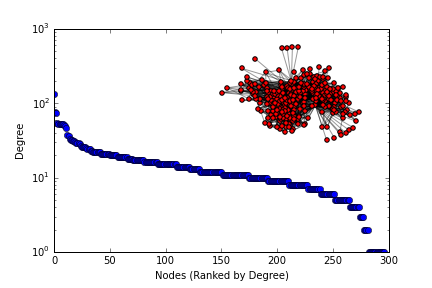
\includegraphics[width=.8\linewidth]{neural_degree_histogram.png}
\caption{Neural Network of \textit{C. Elegans}}
  
\end{figure}

\begin{figure}[H]
\centering
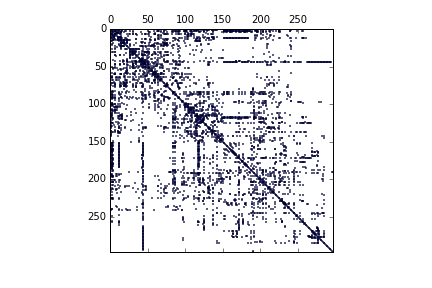
\includegraphics[width = \linewidth]{neuralspy.png}
\caption{Spy Plot of Neural Network Laplacian Matrix}
\end{figure}
\begin{figure}[H]
\centering
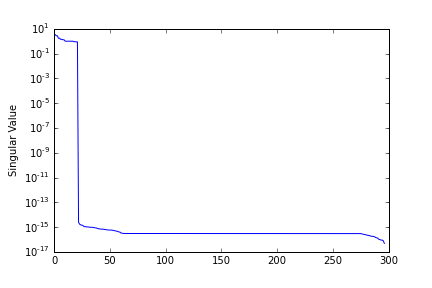
\includegraphics[width = .9\linewidth]{neuralsing.png}
\end{figure}


\subsection{\textit{C. Elegans} Metabolic Network}
\begin{figure}[H]
\centering

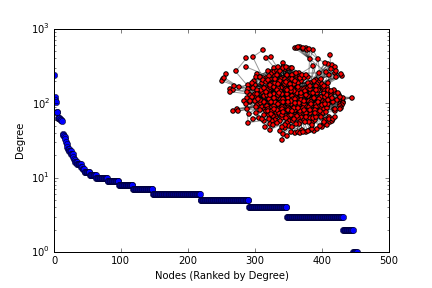
\includegraphics[width=.8\linewidth]{meta_degree_histogram.png}
\caption{Metabolic Network of \textit{C. Elegans}}
  
\end{figure}
\begin{figure}[H]
\centering
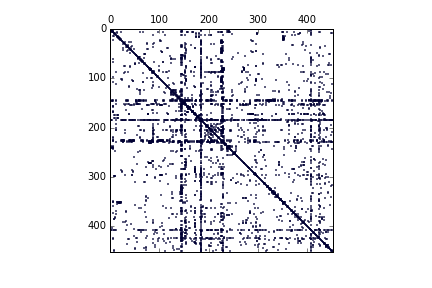
\includegraphics[width = \linewidth]{metaspy.png}
\caption{Spy Plot of Metabolic Network Laplacian Matrix}
\end{figure}
\begin{figure}[H]
\centering
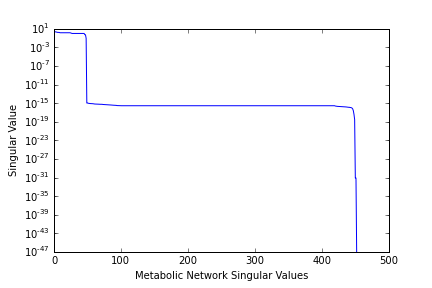
\includegraphics[width = .9\linewidth]{metasing.png}
\end{figure}


\subsection{\textit{C. Elegans} Protein Network}
\begin{figure}[H]
\centering

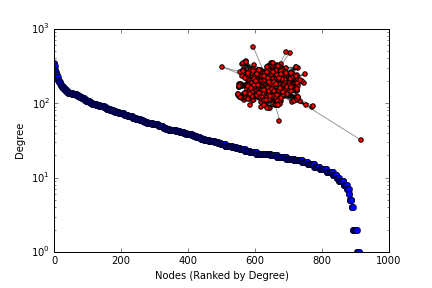
\includegraphics[width=.8\linewidth]{gene_degree_histogram.png}
\caption{Protein Network with Corresponding Phenotypes of \textit{C. Elegans}}
  
\end{figure}

\begin{figure}[H]
\centering
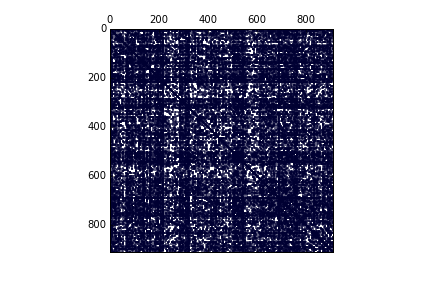
\includegraphics[width = \linewidth]{genespy.png}
\caption{Spy Plot of Protein Network Laplacian Matrix}
\end{figure}
\begin{figure}[H]
\centering
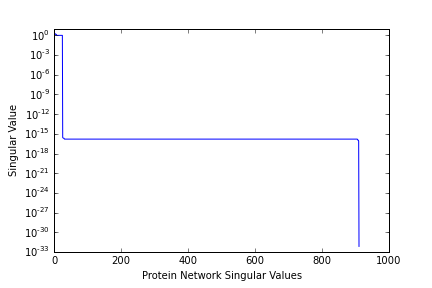
\includegraphics[width = .9\linewidth]{proteinsing.png}
\end{figure}


\subsection{Facebook Friend Network}
\begin{figure}[H]
\centering

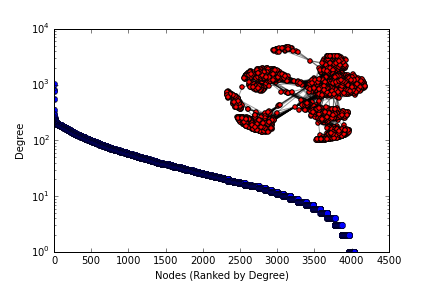
\includegraphics[width=.8\linewidth]{fb_degree_histogram.png}
\caption{Facebook Friend Network}
  
\end{figure}

\begin{figure}[H]
\centering
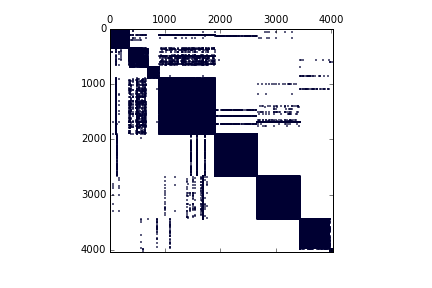
\includegraphics[width = \linewidth]{fbspy.png}
\caption{Spy Plot of Facebook Network Laplacian Matrix}
\end{figure}
\begin{figure}[H]
\centering
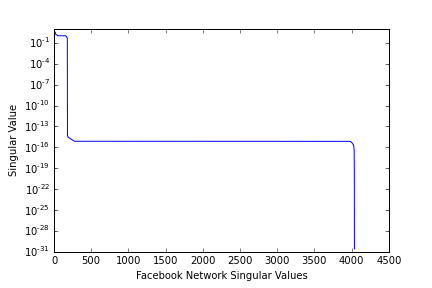
\includegraphics[width = .9\linewidth]{fbsing.png}
\end{figure}


\subsection{Power Grid}

\begin{figure}[H]
\centering

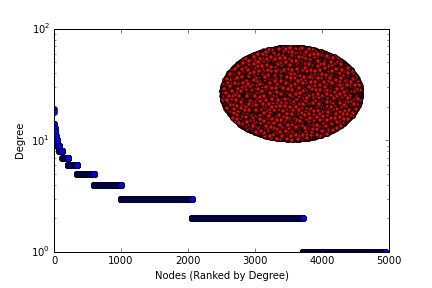
\includegraphics[width=.8\linewidth]{power_degree_histogram.png}
\caption{Network of Western Power Grid}
  
\end{figure}

\begin{figure}[H]
\centering
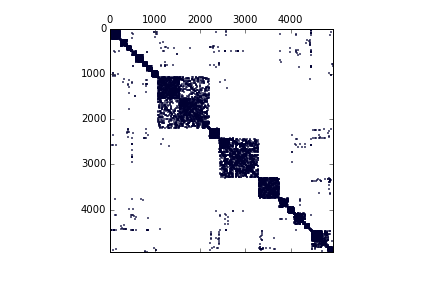
\includegraphics[width = \linewidth]{powerspy.png}
\caption{Spy Plot of Power Grid Laplacian Matrix}
\end{figure}

\begin{figure}[H]
\centering
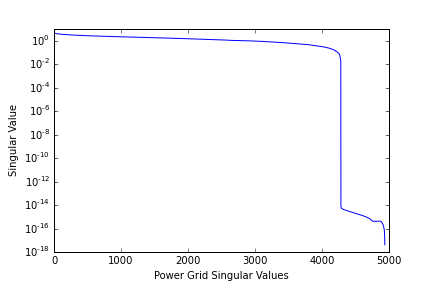
\includegraphics[width = .9\linewidth]{powersing.png}
\end{figure}

\end{document}
